\subsection{QuizziPedia::Back-End::App::Controllers}
\subsubsection{Informazioni generali}
\label{QuizziPedia::Back-End::App::Controllers}
\begin{figure}[ht]
	\centering
	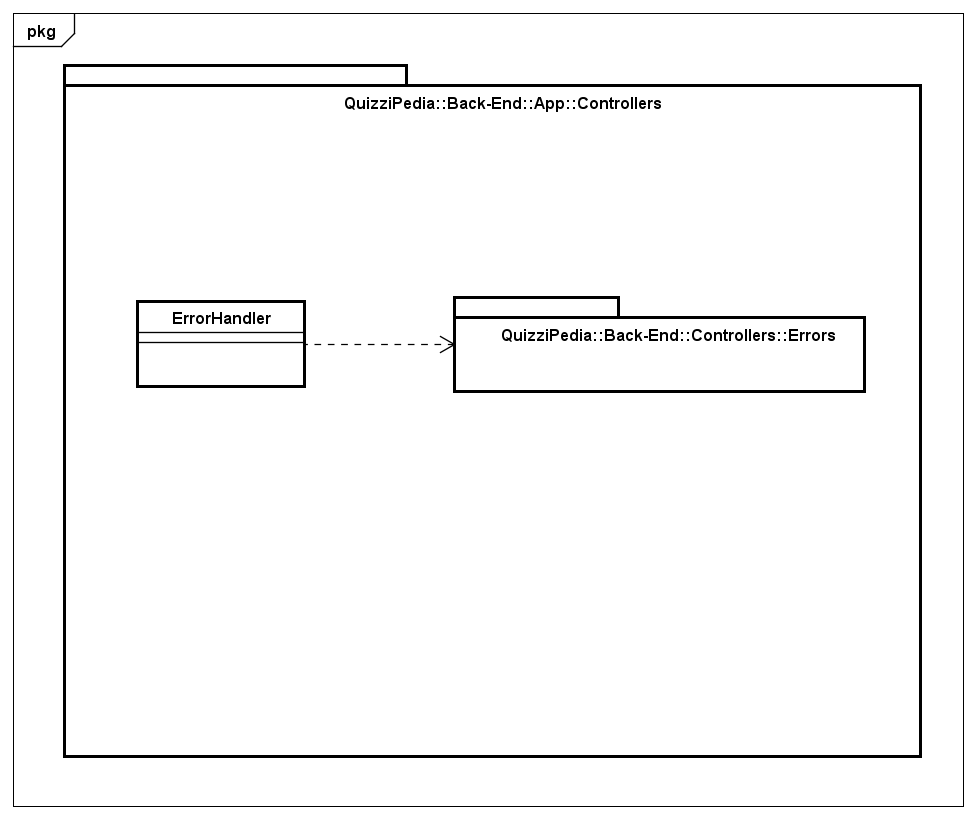
\includegraphics[scale=0.6]{UML/Package/QuizziPedia_Back-End_App_Controllers.png}
	\caption{QuizziPedia::Back-End::App::Controllers}
\end{figure}
\FloatBarrier
	\begin{itemize}
		\item \textbf{Descrizione}:
		\textit{package\ped{G}} contenente i \textit{controllers} di \textit{Express\ped{G}}, definisce la logica dell'applicazione;
		\item \textbf{Padre}: \texttt{App};
		\item \textbf{Interazioni con altri componenti}:
			\begin{itemize}
				\item \texttt{Routers}:
				\textit{package\ped{G}} contenente i router della componente back-end dell'applicazione. Contiene i file di configurazione relativi al routing delle richieste del \textit{client\ped{G}}, ossia i \textit{routers} di \textit{Express\ped{G}};
				\item \texttt{Views}:
				\textit{package\ped{G}} contenente le \textit{\textit{views\ped{G}}} della componente back-end dell'applicazione.
			\end{itemize}
		\item \textbf{Package contenuti}:
			\begin{itemize}
				\item \texttt{Errors}:
				\textit{package\ped{G}} contenente i \textit{controllers} per la gestione degli errori specifici.
			\end{itemize}
	\end{itemize}
\subsubsection{Classi}
\paragraph{QuizziPedia::Back-End::App::Controllers::ErrorsHandler}
\begin{figure}[ht]
	\centering
	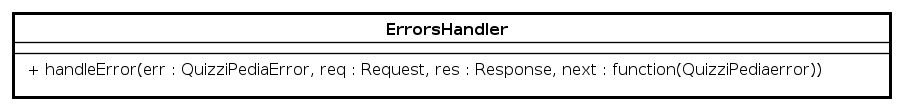
\includegraphics[scale=0.6]{UML/Classi/Back-End/QuizziPedia_Back-End_App_Controllers_ErrorsHandler.png}
	\caption{QuizziPedia::Back-End::App::Controllers::ErrorsHandler}
\end{figure}
\FloatBarrier


\begin{itemize}
	\item \textbf{Descrizione}:
	classe \textit{middleware\ped{G}} per la gestione degli errori. Ritorna al client un oggetto di tipo \texttt{Response} con stato \textit{HTTP\ped{G}} 500 e descrizione dell'errore in formato \textit{JSON\ped{G}}. È un componente \textit{ConcreteHandler\ped{G}} del \textit{design pattern\ped{G}} \textit{Chain of responsibility\ped{G}};
	\item \textbf{Utilizzo}:
	viene utilizzata quando si verifica un errore. Si preoccupa di delegare la costruzione del messaggio d'errore al modulo specifico qualora questo esista, altrimenti costruisce un messaggio d'errore generico. In questo modo i messaggi d'errore specifici vengono delegati ad un altro modulo, rendendo così possibile aggiungere in futuro altri moduli per gestire più flessibilmente nuove tipologie di errori;
	\item \textbf{Relazioni con altre classi}:
	\begin{itemize}
		\item \textbf{IN \texttt{QuizRouter}}:
		classe che gestisce le richieste relative alla gestione di un questionario. Componente \textit{ConcreteHandler\ped{G}} del \textit{design pattern\ped{G}} \textit{Chain of responsibility\ped{G}};
		\item \textbf{IN \texttt{QuestionRouter}}:
		classe che gestisce le richieste relative alla gestione di una domanda. Componente \textit{ConcreteHandler\ped{G}} del \textit{design pattern\ped{G}} \textit{Chain of responsibility\ped{G}};
		\item \textbf{IN \texttt{UserRouter}}:
		classe che gestisce le richieste relative alla gestione di un utente. Componente \textit{ConcreteHandler\ped{G}} del \textit{design pattern\ped{G}} \textit{Chain of responsibility\ped{G}}; Utilizza il modulo \textit{Passport\ped{G}};
		\item \textbf{OUT \texttt{QuizziPediaError}}:
		classe di gestione degli errori. Esegue la costruzione del messaggio d'errore specifico per i moduli di QuizziPedia::Back-End::App.
	\end{itemize}
	\item \textbf{Metodi}:
	\begin{itemize}
		\item \texttt{+ handleError(err: QuizziPediaError, req: Request, res: Response, \\next: function(QuizziPediaError)):void}\\
		Metodo che gestisce la costruzione dei messaggi d'errore ritornando un \textit{JSON\ped{G}} contenente il messaggio d'errore.\\
		\textbf{Parametri}:
		\begin{itemize}
			\item \texttt{err: QuizziPediaError}\\
			Rappresenta l'errore di tipo \texttt{QuizziPediaError};
			\item \texttt{req: Request}\\
			Rappresenta la richiesta inviata al \textit{server\ped{G}};
			\item \texttt{res: Response}\\
			Rappresenta la risposta che il \textit{server\ped{G}} fornirà al termine dell'esecuzione del metodo;
			\item \texttt{next: function(QuizziPediaError)}\\
			Rappresenta la \textit{callback\ped{G}} che il metodo deve chiamare al termine dell'elaborazione per passare il controllo ai successivi \textit{middleware\ped{G}}. La presenza del parametro facoltativo \texttt{QuizziPediaError} attiva la catena di gestione dell'errore in sostituzione della normale catena di gestione delle richieste.
		\end{itemize}
		\item \texttt{+ insertError(req: Request, res: Response, \\next: function(QuizziPediaError)):void}\\
		Metodo che inserisce una nuova tipologia di errore all'interno del database.\\
		\textbf{Parametri}:
		\begin{itemize}
			\item \texttt{req: Request}\\
			Rappresenta la richiesta inviata al \textit{server\ped{G}}; contiene i dati della nuova tipologia di errore che si vuole inserire nel database;
			\item \texttt{res: Response}\\
			Rappresenta la risposta che il \textit{server\ped{G}} fornirà al termine dell'esecuzione del metodo;
			\item \texttt{next: function(QuizziPediaError)}\\
			Rappresenta la \textit{callback\ped{G}} che il metodo deve chiamare al termine dell'elaborazione per passare il controllo ai successivi \textit{middleware\ped{G}}. La presenza del parametro facoltativo \texttt{QuizziPediaError} attiva la catena di gestione dell'errore in sostituzione della normale catena di gestione delle richieste.
		\end{itemize}
	\end{itemize}
\end{itemize}

\paragraph{QuizziPedia::Back-End::App::Controllers::TopicController}
\label{QuizziPedia::Back-End::App::Controllers::TopicController}
\begin{figure}[ht]
	\centering
	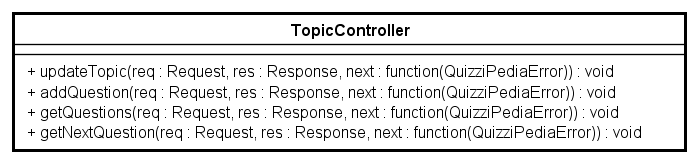
\includegraphics[scale=0.6]{UML/Classi/Back-End/QuizziPedia_Back-End_App_Controllers_topicController.png}
	\caption{QuizziPedia::Back-End::App::Controllers::TopicController}
\end{figure}
\FloatBarrier
\begin{itemize}
	\item \textbf{Descrizione}:
	classe che gestisce la logica applicativa riguardante la visualizzazione e la modifica degli argomenti delle domande;
	\item \textbf{Utilizzo}:
	viene utilizzata per implementare le funzionalità necessarie a gestire le richieste \textit{REST\ped{G}} legate agli argomenti delle domande;
	\item \textbf{Relazioni con altre classi}:
		\begin{itemize}
			\item \textbf{IN \texttt{QuestionRouter}}:
			classe che gestisce le richieste relative alle operazioni riguardanti le domande. Componente \textit{ConcreteHandler\ped{G}} del \textit{design pattern\ped{G}} \textit{Chain of responsibility\ped{G}};
			\item \textbf{OUT \texttt{TopicModel}}: 
			classe che modella gli argomenti delle domande.
		\end{itemize}
	\item \textbf{Metodi}:
		\begin{itemize}
			\item \texttt{+ updateStatisticTopic(req : Request, res : Response, \\next : function(QuizziPediaError)): void} \\
			Aggiorna il numero di risposte esatte e totali date a domande sull'argomento da parte degli utenti. \\
			\textbf{Parametri}:
			\begin{itemize}
			\item \texttt{req: Request} \\
			Rappresenta la richiesta inviata al \textit{server\ped{G}}. Contiene l'identificativo dell'argomento da aggiornare e l'informazione di se è stata data o meno una risposta corretta alla domanda su quell'argomento;
			\item \texttt{res: Response} \\
			Rappresenta la risposta che il \textit{server\ped{G}} fornirà al termine dell'esecuzione del metodo;
			\item \texttt{next: function(QuizziPediaError)} \\
			Rappresenta la \textit{callback\ped{G}} che il metodo deve chiamare al termine dell'elaborazione per passare il controllo ai successivi \textit{middleware\ped{G}}. La presenza del parametro facoltativo QuizziPediaError attiva la catena di gestione dell'errore in sostituzione della normale catena di gestione delle richieste.
			\end{itemize}
			\item \texttt{+ getNextQuestion(req : Request, \\res : Response, next : function(QuizziPediaError)): void} \\
			Restituisce la domanda successiva di un allenamento.  \\
			\textbf{Parametri}:
			\begin{itemize}
			\item \texttt{req: Request} \\
			Rappresenta la richiesta inviata al \textit{server\ped{G}}. Contiene l'identificativo dell'argomento trattato nell'allenamento e il livello dell'utente che lo sta svolgendo;
			\item \texttt{res: Response} \\
			Rappresenta la risposta che il \textit{server\ped{G}} fornirà al termine dell'esecuzione del metodo;
			\item \texttt{next: function(QuizziPediaError)} \\
			Rappresenta la \textit{callback\ped{G}} che il metodo deve chiamare al termine dell'elaborazione per passare il controllo ai successivi \textit{middleware\ped{G}}. La presenza del parametro facoltativo QuizziPediaError attiva la catena di gestione dell'errore in sostituzione della normale catena di gestione delle richieste.
			\end{itemize}
			\item \texttt{+ getTopics(req : Request, \\res : Response, next : function(QuizziPediaError)): void} \\
			Restituisce gli argomenti presenti nel sistema.  \\
			\textbf{Parametri}:
			\begin{itemize}
			\item \texttt{req: Request} \\
			Rappresenta la richiesta inviata al \textit{server\ped{G}};
			\item \texttt{res: Response} \\
			Rappresenta la risposta che il \textit{server\ped{G}} fornirà al termine dell'esecuzione del metodo;
			\item \texttt{next: function(QuizziPediaError)} \\
			Rappresenta la \textit{callback\ped{G}} che il metodo deve chiamare al termine dell'elaborazione per passare il controllo ai successivi \textit{middleware\ped{G}}. La presenza del parametro facoltativo QuizziPediaError attiva la catena di gestione dell'errore in sostituzione della normale catena di gestione delle richieste.
			\end{itemize}
			\item \texttt{+ getKeywords(req : Request, \\res : Response, next : function(QuizziPediaError)): void} \\
			Restituisce tutte le keywords delle domande di un singolo argomento.  \\
			\textbf{Parametri}:
			\begin{itemize}
			\item \texttt{req: Request} \\
			Rappresenta la richiesta inviata al \textit{server\ped{G}};
			\item \texttt{res: Response} \\
			Rappresenta la risposta che il \textit{server\ped{G}} fornirà al termine dell'esecuzione del metodo;
			\item \texttt{next: function(QuizziPediaError)} \\
			Rappresenta la \textit{callback\ped{G}} che il metodo deve chiamare al termine dell'elaborazione per passare il controllo ai successivi \textit{middleware\ped{G}}. La presenza del parametro facoltativo QuizziPediaError attiva la catena di gestione dell'errore in sostituzione della normale catena di gestione delle richieste.
			\end{itemize}
		\end{itemize}
\end{itemize}
\paragraph{QuizziPedia::Back-End::App::Controllers::SummaryController}
\label{QuizziPedia::Back-End::App::Controllers::SummaryController}
\begin{figure}[ht]
	\centering
	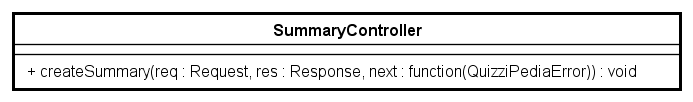
\includegraphics[scale=0.45]{UML/Classi/Back-End/QuizziPedia_Back-End_App_Controllers_SummaryController.png}
	\caption{QuizziPedia::Back-End::App::Controllers::SummaryController}
\end{figure}
\FloatBarrier

\begin{itemize}
	\item \textbf{Descrizione} \\
	Classe che gestisce la logica applicativa riguardante la visualizzazione e la modifica dei riepiloghi dei questionari.
	\item \textbf{Utilizzo} \\
	Viene utilizzata per implementare le funzionalità necessarie a gestire le richieste \textit{REST\ped{G}} legate ai riepiloghi dei questionari.
	\item \textbf{Relazione con altre classi}\\
	\begin{itemize}
			\item \textbf{IN \texttt{UserRouter}} \\
			Classe che gestisce le richieste relative alla registrazione, alla gestione della sessione e alla cronologia dei questionari svolti di un utente;
			\item \textbf{OUT \texttt{SummaryModel}} \\
			Classe che modella i riepiloghi dei questionari.
	\end{itemize}
	\item \textbf{Metodi}\\
	\begin{itemize}
		\item \texttt{+ createSummary(req: Request, res: Response, next: \\function(QuizziPediaError))}\\
		Crea un riepilogo.\\
		\textbf{Parametri}:
		\begin{itemize}
			\item \texttt{req: Request}\\
			Rappresenta la richiesta inviata al \textit{server\ped{G}}. Contiene l'identificativo del questionario per cui verrà creato il riepilogo e le risposte date alle domande;
			\item \texttt{res: Response}\\
			Rappresenta la risposta che il \textit{server\ped{G}} fornirà al termine dell'esecuzione del metodo;
			\item \texttt{next: function(QuizziPediaError)}\\
			Rappresenta la \textit{callback\ped{G}} che il metodo deve chiamare al termine dell'elaborazione per passare il controllo ai successivi \textit{middleware\ped{G}}. La presenza del parametro facoltativo \texttt{QuizziPediaError} attiva la catena di gestione dell'errore in sostituzione della normale catena di gestione delle richieste.
		\end{itemize}
	\end{itemize}
\end{itemize}
\paragraph{QuizziPedia::Back-End::App::Controllers::QuizController}
\label{QuizziPedia::Back-End::App::Controllers::QuizController}
\begin{figure}[ht]
	\centering
	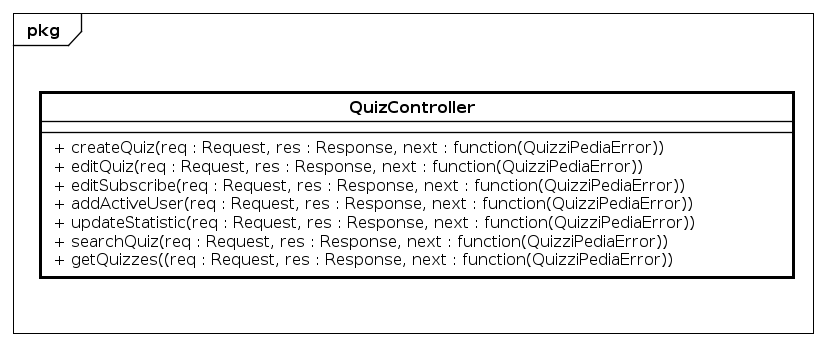
\includegraphics[scale=0.45]{UML/Classi/Back-End/QuizziPedia_Back-End_App_Controllers_quizController.png}
	\caption{QuizziPedia::Back-End::App::Models::Controllers::TopicController}
\end{figure}
\FloatBarrier

\begin{itemize}
	\item \textbf{Descrizione} \\
	Classe che gestisce la logica applicativa riguardante la visualizzazione e la gestione dei questionari.
	\item \textbf{Utilizzo} \\
	Viene utilizzata per implementare le funzionalità necessarie a gestire le richieste \textit{REST\ped{G}} legate alla gestione dei questionari.
	\item \textbf{Relazione con altre classi}\\
	\begin{itemize}
			\item \textbf{IN \texttt{QuizRouter}}\\
			Classe che gestisce le richieste relative alle operazioni riguardanti un questionario;
			\item \textbf{OUT \texttt{QuizModel}} \\
			Classe che modella i questionari.
	\end{itemize}
	\item \textbf{Metodi}\\
	\begin{itemize}
		\item \texttt{+ createQuiz(req: Request, res: Response, next: function(QuizziPediaError))}\\
		Crea un questionario.\\
		\textbf{Parametri}:
		\begin{itemize}
			\item \texttt{req: Request}\\
			Rappresenta la richiesta inviata al \textit{server\ped{G}}. Contiene i dati che verranno utilizzati per creare il questionario e gli identificativi delle domande che verranno inserite;
			\item \texttt{res: Response}\\
			Rappresenta la risposta che il \textit{server\ped{G}} fornirà al termine dell'esecuzione del metodo;
			\item \texttt{next: function(QuizziPediaError)}\\
			Rappresenta la \textit{callback\ped{G}} che il metodo deve chiamare al termine dell'elaborazione per passare il controllo ai successivi \textit{middleware\ped{G}}. La presenza del parametro facoltativo \texttt{QuizziPediaError} attiva la catena di gestione dell'errore in sostituzione della normale catena di gestione delle richieste.
		\end{itemize}
	
	\item \texttt{+ editQuiz(req: Request, res: Response, next: function(QuizziPediaError))}\\
		Modifica un questionario secondo i dati inseriti dall'utente.\\
		\textbf{Parametri}:
		\begin{itemize}
			\item \texttt{req: Request}\\
			Rappresenta la richiesta inviata al \textit{server\ped{G}}. Contiene le modifiche apportate dall'utente e l'identificativo del questionario su cui verranno applicate;
			\item \texttt{res: Response}\\
			Rappresenta la risposta che il \textit{server\ped{G}} fornirà al termine dell'esecuzione del metodo;
			\item \texttt{next: function(QuizziPediaError)}\\
			Rappresenta la \textit{callback\ped{G}} che il metodo deve chiamare al termine dell'elaborazione per passare il controllo ai successivi \textit{middleware\ped{G}}. La presenza del parametro facoltativo \texttt{QuizziPediaError} attiva la catena di gestione dell'errore in sostituzione della normale catena di gestione delle richieste.
		\end{itemize}
		
		\item \texttt{+ editSubscribe(req: Request, res: Response, next: function(QuizziPediaError))}\\
		Modifica le iscrizioni al questionario.\\
		\textbf{Parametri}:
		\begin{itemize}
			\item \texttt{req: Request}\\
			Rappresenta la richiesta inviata al \textit{server\ped{G}}. Contiene l'identificativo del questionario la cui lista delle iscrizioni deve essere modificata;
			\item \texttt{res: Response}\\
			Rappresenta la risposta che il \textit{server\ped{G}} fornirà al termine dell'esecuzione del metodo;
			\item \texttt{next: function(QuizziPediaError)}\\
			Rappresenta la \textit{callback\ped{G}} che il metodo deve chiamare al termine dell'elaborazione per passare il controllo ai successivi \textit{middleware\ped{G}}. La presenza del parametro facoltativo \texttt{QuizziPediaError} attiva la catena di gestione dell'errore in sostituzione della normale catena di gestione delle richieste.
		\end{itemize}
		
		\item \texttt{+ addActiveUser(req: Request, res: Response, next: function(QuizziPediaError))}\\
		Aggiorna la lista di utenti che hanno svolto il questionario.\\
		\textbf{Parametri}:
		\begin{itemize}
			\item \texttt{req: Request}\\
			Rappresenta la richiesta inviata al \textit{server\ped{G}}. Contiene l'identificativo del questionario la cui lista delle iscrizioni deve essere modificata;
			\item \texttt{res: Response}\\
			Rappresenta la risposta che il \textit{server\ped{G}} fornirà al termine dell'esecuzione del metodo;
			\item \texttt{next: function(QuizziPediaError)}\\
			Rappresenta la \textit{callback\ped{G}} che il metodo deve chiamare al termine dell'elaborazione per passare il controllo ai successivi \textit{middleware\ped{G}}. La presenza del parametro facoltativo \texttt{QuizziPediaError} attiva la catena di gestione dell'errore in sostituzione della normale catena di gestione delle richieste.
		\end{itemize}
		
		\item \texttt{+ updateStatistic(req: Request, res: Response, next: function(QuizziPediaError))}\\
		Aggiorna le statistiche del questionario.\\
		\textbf{Parametri}:
		\begin{itemize}
			\item \texttt{req: Request}\\
			Rappresenta la richiesta inviata al \textit{server\ped{G}}. Contiene l'identificativo del questionario le cui statistiche dovranno essere modificate e i valori da aggiornare;
			\item \texttt{res: Response}\\
			Rappresenta la risposta che il \textit{server\ped{G}} fornirà al termine dell'esecuzione del metodo;
			\item \texttt{next: function(QuizziPediaError)}\\
			Rappresenta la \textit{callback\ped{G}} che il metodo deve chiamare al termine dell'elaborazione per passare il controllo ai successivi \textit{middleware\ped{G}}. La presenza del parametro facoltativo \texttt{QuizziPediaError} attiva la catena di gestione dell'errore in sostituzione della normale catena di gestione delle richieste.
		\end{itemize}
		
		\item \texttt{+ searchQuiz(req: Request, res: Response, next: function(QuizziPediaError))}\\
		Ricerca un questionario.\\
		\textbf{Parametri}:
		\begin{itemize}
			\item \texttt{req: Request}\\
			Rappresenta la richiesta inviata al \textit{server\ped{G}}. Contiene il nome del questionario da ricercare;
			\item \texttt{res: Response}\\
			Rappresenta la risposta che il \textit{server\ped{G}} fornirà al termine dell'esecuzione del metodo;
			\item \texttt{next: function(QuizziPediaError)}\\
			Rappresenta la \textit{callback\ped{G}} che il metodo deve chiamare al termine dell'elaborazione per passare il controllo ai successivi \textit{middleware\ped{G}}. La presenza del parametro facoltativo \texttt{QuizziPediaError} attiva la catena di gestione dell'errore in sostituzione della normale catena di gestione delle richieste.
		\end{itemize}
		
		\item \texttt{+ getChronology((req: Request, res: Response, next: function(QuizziPediaError))}\\
			Mostra la cronologia dei questionari svolti da un utente.\\
			\textbf{Parametri}:
			\begin{itemize}
				\item \texttt{req: Request}\\
			Rappresenta la richiesta inviata al \textit{server\ped{G}}. Contiene il nome del questionario da ricercare;
				\item \texttt{res: Response}\\
			Rappresenta la risposta che il \textit{server\ped{G}} fornirà al termine dell'esecuzione del metodo;
				\item \texttt{next: function(QuizziPediaError)}\\
			Rappresenta la \textit{callback\ped{G}} che il metodo deve chiamare al termine dell'elaborazione per passare il controllo ai successivi \textit{middleware\ped{G}}. La presenza del parametro facoltativo \texttt{QuizziPediaError} attiva la catena di gestione dell'errore in sostituzione della normale catena di gestione delle richieste.
			\end{itemize}
		
		\item \texttt{+ getPersonalQuizzes((req: Request, res: Response, next: function(QuizziPediaError))}\\
			Mostra i questionari creati da un utente.\\
			\textbf{Parametri}:
			\begin{itemize}
				\item \texttt{req: Request}\\
			Rappresenta la richiesta inviata al \textit{server\ped{G}}. Contiene il nome del questionario da ricercare;
				\item \texttt{res: Response}\\
			Rappresenta la risposta che il \textit{server\ped{G}} fornirà al termine dell'esecuzione del metodo;
				\item \texttt{next: function(QuizziPediaError)}\\
			Rappresenta la \textit{callback\ped{G}} che il metodo deve chiamare al termine dell'elaborazione per passare il controllo ai successivi \textit{middleware\ped{G}}. La presenza del parametro facoltativo \texttt{QuizziPediaError} attiva la catena di gestione dell'errore in sostituzione della normale catena di gestione delle richieste.
			\end{itemize}
	\end{itemize}		
\end{itemize}
\paragraph{QuizziPedia::Back-End::App::Controllers::QuestionController}
\label{QuizziPedia::Back-End::App::Controllers::QuestionController}
\begin{figure}
	\centering
	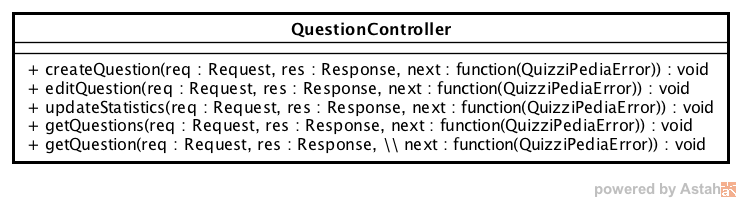
\includegraphics[scale=0.45]{UML/Classi/Back-End/QuizziPedia_Back-End_App_Controllers_questionController.png}
	\caption{QuizziPedia::Back-End::App::Models::Controllers::QuestionController}
\end{figure}
	\begin{itemize}
		\item \textbf{Descrizione} \\
		Classe che gestisce la logica applicativa riguardante la visualizzazione, la creazione e la modifica delle domande presenti nell'applicazione;
		\item \textbf{Utilizzo} \\
		Viene utilizzata per implementare le funzionalità necessarie a gestire le richieste REST\ped{G} legate alle domande;
		\item \textbf{Relazioni con altre classi}
			\begin{itemize}
				\item \textbf{OUT \texttt{QuestionModel}} \\
				Classe che modella le domande dell'applicazione;
			\end{itemize}
		\item \textbf{Metodi}
			\begin{itemize}
				\item \texttt{+ createQuestion(req: Request, res: Response, next: function(QuizziPediaError))} \\
				Crea e aggiunge una nuova domanda nel sistema. \\
				\textbf{Parametri:}
				\begin{itemize}
					\item \texttt{req: Request} \\
					Rappresenta la richiesta inviata al \textit{server\ped{G}}. Contiene l'identificativo dell'utente autenticato.
					\item \texttt{res: Response} \\
					Rappresenta la risposta che il \textit{server\ped{G}} fornirà al termine dell'esecuzione del metodo.
					\item \texttt{next: function(QuizziPediaError)} \\
					Rappresenta la \textit{callback\ped{G}} che il metodo deve chiamare al termine dell'elaborazione per passare il controllo ai successivi \textit{middleware\ped{G}}. La presenza del parametro facoltativo \texttt{QuizziPediaError} attiva la catena di gestione dell'errore in sostituzione della normale catena di gestione delle richieste.
				\end{itemize}
				\item \texttt{+ editQuestion(req: Request, res: Response, next: function(QuizziPediaError))} \\
				Modifica una domanda già esistente nel sistema. \\
				\textbf{Parametri:}
					\begin{itemize}
						\item \texttt{req: Request} \\
						Rappresenta la richiesta inviata al \textit{server\ped{G}}. Contiene l'identificativo dell'utente autenticato. In \texttt{req} è presente un campo che rappresenta l'identificativo della domanda nel database che il metodo deve modificare e le relative modifiche.
						\item \texttt{res: Response} \\
						Rappresenta la risposta che il \textit{server\ped{G}} fornirà al termine dell'esecuzione del metodo.
						\item \texttt{next: function(QuizziPediaError)} \\
						Rappresenta la \textit{callback\ped{G}} che il metodo deve chiamare al termine dell'elaborazione per passare il controllo ai successivi \textit{middleware\ped{G}}. La presenza del parametro facoltativo \texttt{QuizziPediaError} attiva la catena di gestione dell'errore in sostituzione della normale catena di gestione delle richieste.
					\end{itemize}
				\item \texttt{+ updateStatistic(req: Request, res: Response, next: function(QuizziPediaError))} \\
				Aggiorna le statistiche sulla difficoltà della domanda, aggiornando anche i campi relativi al numero di risposte totali date alla domanda e al numero di risposte corrette ad ogni risposta da parte di un utente. \\
				\textbf{Parametri:}
					\begin{itemize}
						\item \texttt{req: Request} \\
						Rappresenta la richiesta inviata al \textit{server\ped{G}}. Contiene l'identificativo della domanda, il livello dell'utente che ha risposto e se è stata data la risposta corretta.
						\item \texttt{res: Response} \\
						Rappresenta la risposta che il \textit{server\ped{G}} fornirà al termine dell'esecuzione del metodo.
						\item \texttt{next: function(QuizziPediaError)} \\
						Rappresenta la \textit{callback\ped{G}} che il metodo deve chiamare al termine dell'elaborazione per passare il controllo ai successivi textit{middleware\ped{G}}. La presenza del parametro facoltativo \texttt{QuizziPediaError} attiva la catena di gestione dell'errore in sostituzione della normale catena di gestione delle richieste.
					\end{itemize}
			\end{itemize}
	\end{itemize}
\paragraph{QuizziPedia::Back-End::App::Controllers::UserController}
\label{QuizziPedia::Back-End::App::Controllers::UserController}
\begin{figure}[ht]
	\centering
	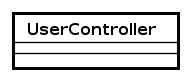
\includegraphics[scale=0.45]{UML/Classi/Back-End/QuizziPedia_Back-End_App_Controllers_UserController.png}
	\caption{QuizziPedia::Back-End::App::Controllers::UserController}
\end{figure}
\FloatBarrier
\begin{itemize}
	\item 
	\textbf{Descrizione}:\\
	Classe che raggruppa attraverso require i vari controllers responsabili delle operazioni legate alla gestione degli utenti. Si è scelto di predisporre questo raggruppamento per facilitare l'introduzione di nuove funzionalità legate alla gestione degli utenti.
	\item \textbf{Utilizzo}:\\
	Viene utilizzata per raggruppare i controllers responsabili della gestione dei dati degli utenti. In questo modo le classi che vogliono comunicare con i controllers legati agli utenti necessitano di includere solo questa classe e non ogni singolo controller.
	\item \textbf{Relazioni con altre classi}:
	\begin{itemize}
		\item 
			IN	\texttt{UserRouter}\\
			Classe che gestisce le richieste relative alla registrazione e alla gestione della sessione di un utente. Componente ConcreteHandler del design pattern \textit{Chain of responsibility\ped{G}}. Utilizza il modulo \textit{Passport\ped{G}}.		
		\item 
			OUT \texttt{SessionController}\\
			Classe \textit{middleware\ped{G}} che, utilizzando \textit{Passport\ped{G}}, si occupa di controllare la consistenza dell'oggetto session durante la sessione associata all'utente autenticato. È un componente ConcreteHandler del design pattern \textit{Chain of responsibility\ped{G}}.
		\item 
			OUT \texttt{AuthenticationController}\\
			Classe che si occupa della registrazione e dell'autenticazione dell'utente nel sistema. È un componente ConcreteHandler del design pattern \textit{Chain of responsibility\ped{G}}. Risulta essere il componente che eventualmente esegue la richiesta del client attraverso \textit{Passport\ped{G}}.	
		\item 
			OUT \texttt{UserManagementController}\\
			Classe che gestisce la logica applicativa riguardante la visualizzazione e la modifica dei dati dell'utente.
			Rappresenta il ConcreteHandler nel design pattern \textit{Chain of responsibility\ped{G}}. Utilizza \textit{Passport\ped{G}}.
	\end{itemize}
\end{itemize}

\paragraph{QuizziPedia::Back-End::App::Controllers::LangController}
\label{QuizziPedia::Back-End::App::Controllers::UserController}
\begin{figure}[ht]
	\centering
	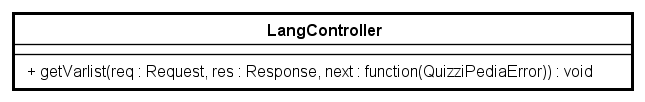
\includegraphics[scale=0.45]{UML/Classi/Back-End/QuizziPedia_Back-End_App_Controllers_langController.png}
	\caption{QuizziPedia::Back-End::App::Controllers::LangController}
\end{figure}
\FloatBarrier
\begin{itemize}
	\item 
	\textbf{Descrizione}:\\
	Classe che gestisce la logica applicativa riguardante il passaggio della traduzione delle variabili;
	\item \textbf{Utilizzo}:\\
	Viene utilizzata per gestire la richiesta di traduzione delle variabili;
	\item \textbf{Relazioni con altre classi}:
	\begin{itemize}
		\item IN LangModel \\
		Classe che modella le informazioni riguardanti la lingua dell'applicazione;
	\end{itemize}
	\item \textbf{Metodi}:
		\begin{itemize}
			\item \texttt{+ getVarlist(req: Request, res: Response, next: function(QuizziPediaError))} \\
			\textbf{Parametri}:
				\begin{itemize}
					\item \texttt{req: Request} \\
					Rappresenta la richiesta inviata al server\ped{G}. Contiene la stringa che indica la lingua che si vuole tradurre le variabili;
					\item \texttt{res: Response} \\
					Rappresenta la risposta che il server fornirà al termine  dell'esecuzione del metodo;
					\item \texttt{next: function(QuizziPediaError)} \\
					Rappresenta la \textit{callback\ped{G}} che il metodo deve chiamare al termine dell'elaborazione per passare il controllo ai successivi \textit{middleware\ped{G}}. La presenza del parametro facoltativo \textit{QuizziPediaError} attiva la catena di gestione dell'errore in sostituzione della normale catena di gestione delle richieste;
				\end{itemize}
		\end{itemize}
\end{itemize}

\subsection{QuizziPedia::Back-End::App::Controllers::NotFoundHandler}
\subsubsection{Informazioni generali}
\label{QuizziPedia::Back-End::App::Controllers::NotFoundHandler}
%\begin{figure}
%	\centering
%	\includegraphics[scale=0.45]{UML/Package/.............creare immagine........}
%	\caption{QuizziPedia::Back-End::App::Controllers::NotFoundHandler}
%\end{figure}

\begin{itemize}
	\item \textbf{Descrizione}\\
	Classe che si occupa della gestione dell'errore di pagina non trovata. Componente ConcreteHandler del design pattern Chain of responsibility.
	\item \textbf{Utilizzo}\\
	Viene utilizzata per generare una pagina 404 di errore nel caso in cui l'URI passato non corrisponda ad una risorsa presente nell'applicazione.
	\item \textbf{Relazione con altre classi}\\
	\begin{itemize}
		\item \textbf{IN} \texttt{UserRouter}\\
		Classe che gestisce le richieste relative alle operazioni riguardanti l'utente. Componente ConcreteHandler del design pattern Chain of responsibility.
		\item \textbf{IN} \texttt{QuestionRouter}\\
		Classe che gestisce le richieste relative alle operazioni riguardanti le domande. Componente ConcreteHandler del design pattern Chain of responsibility.
		\item \textbf{IN} \texttt{QuizRouter}\\
		Classe che gestisce le richieste relative alle operazioni riguardanti i questionari. Componente ConcreteHandler del design pattern Chain of responsibility.
		.................................
	\end{itemize}
	\item \textbf{Metodi}\\
	\begin{itemize}
		\item \texttt{+ handle(req: Request, res: Response, next: function(QuizziPediaError))}\\
		Metodo che gestisce la costruzione dei messaggi d'errore ritornando un JSON contenente il messaggio d'errore.\\
		\textbf{Parametri}:
		\begin{itemize}
			\item \texttt{req: Request}\\
			Rappresenta la richiesta inviata al server.
			\item \texttt{res: Response}\\
			Rappresenta la risposta che il server fornirà al termine dell'esecuzione del metodo.
			\item \texttt{next: function(QuizziPediaError)}\\
			Rappresenta la \textit{callback\ped{G}} che il metodo deve chiamare al termine dell'elaborazione per passare il controllo ai successivi middleware. La presenza del parametro facoltativo QuizziPediaError attiva la catena di gestione dell'errore in sostituzione della normale catena di gestione delle richieste.
		\end{itemize}
	\end{itemize}
\end{itemize}





